\begin{figure}[h!]
    \centering
    \setlength{\resLen}{1.4in}
    \addtolength{\tabcolsep}{-3.5pt}
    %
    \begin{tabular}{cccc}
        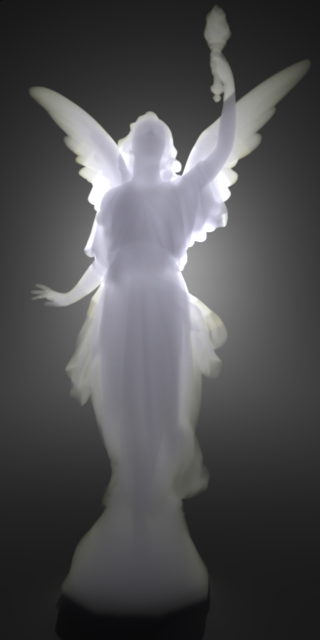
\includegraphics[width=\resLen]{waveoptics/lucy/color.jpg} &
        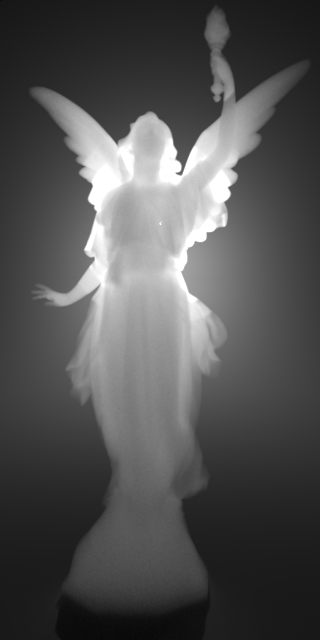
\includegraphics[width=\resLen]{waveoptics/lucy/color_400nm.jpg} &
        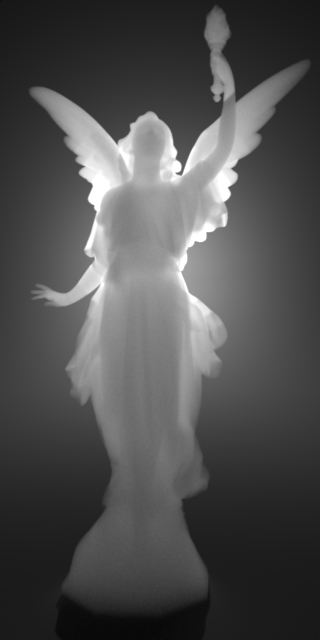
\includegraphics[width=\resLen]{waveoptics/lucy/color_550nm.jpg} &
        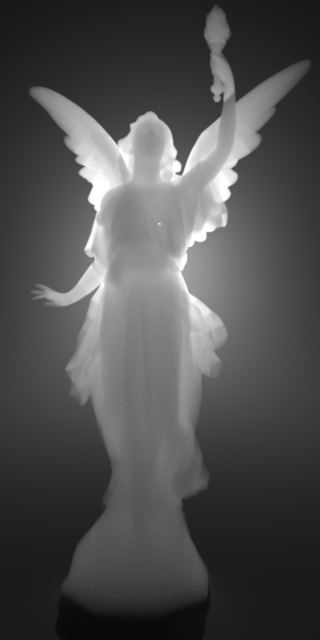
\includegraphics[width=\resLen]{waveoptics/lucy/color_700nm.jpg}
        \\
        \textbf{(a)} Multi. & \textbf{(b)} 400nm & \textbf{(c)} 550nm & \textbf{(d)} 700nm
    \end{tabular}
    \caption[Multi-spectral rendering of homogeneous Lucy model]{\label{fig:waveoptics:multiwave2}
        \textbf{Multi-spectral rendering of Lucy model.} \textbf{(a)} Multi-spectral rendering of a homogeneous Lucy model using identical bulk scattering parameters as the top row of Figure \ref{fig:waveoptics:multiwave1}.
        \textbf{(b--d)} Monochrome renderings of the same model at three wavelengths.
    }
\end{figure}
